\section{FairTest}
\label{sect:fairtest}

% What we built

\begin{figure}[h]
 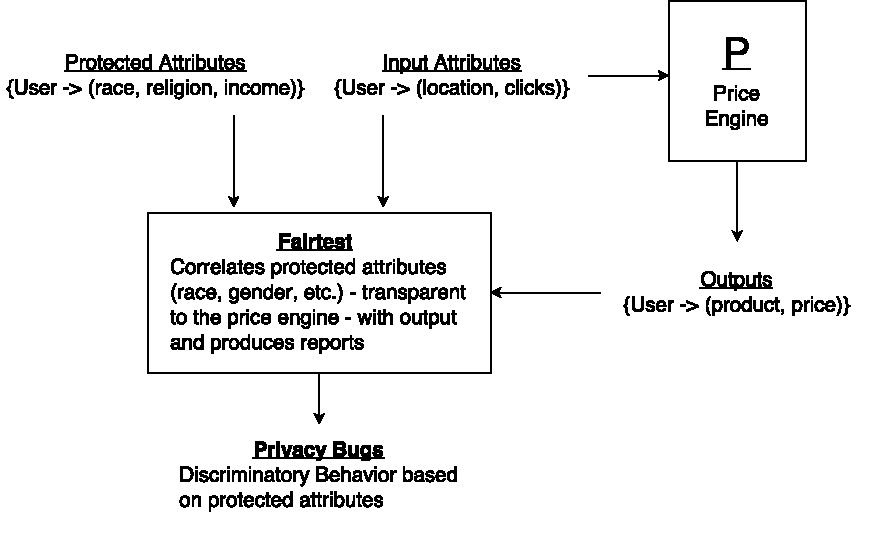
\includegraphics[width=0.49\textwidth]
  {\detokenize{figures/overview}}
  \caption{ {\bf \textit{FairTest} Use Overview}. Gives an overview of how an application
    may use \sysname to generate bug-reports.
  }
  \label{fig:FairtestOverview}
\end{figure}

In this section we present the design and implementation of \sysname.
At its core, \sysname assets that there are no violations of statistical
condition~\ref{eq:StatisticalParity} of Section~\ref{sect:statparity}.
%To address the descrimination test, We designed \textit{FairTest}, a software
%testing framework for web-based applications to find out potential
%\textit{privacy bugs}, whose definition was just described. Its basic workflow
Figure~\ref{fig:FairtestOverview}, gives an overview of how a data-driven
application with a pricing policy ``P'' can use \sysname to generate
bug reports. As shown in Figure~\ref{fig:FairtestOverview}, user-attributes
(protected and non-protected) and price engine's output are used by
\sysname to generate bug-reports. \sysname generates these report based on
on the {\em statistical parity} of users on certain protected attributes
(such as gender, race, etc.). In specific, any violation of
condition~\ref{eq:StatisticalParity}, is reported by \sysname as a {\em privacy bug}.

% Target user / characteristic

\sysname is designed to be used for designers and engineers of 
data-based web applications. In addition, it can also be used for auditors 
or government agencies to look for evidence on certain parity violation,
such as in the Staples case. The framework, for generality, is interfaced 
with RESTful API that can easily connect to existing software solutions.
We expect that developers will only make minimal modifications to the
application (mostly adding the tracking code) to derive the data for audit
in \sysname. Also, to address privacy on the testing framework,
\sysname does not require identifiable user information, such as
exact address, name, etc. The framework itself is implemented in Python and
Django, with support to both SQLite or PostgreSQL database.

% Data got

Once \textit{FairTest} has information about the users and the corresponding
outputs from the software being tested, it can generate statistical reports
evaluating the statistical parity between the protected info, the actual
input and the output. This info can then be reported either through a RESTful
API or a web interface to the developer or tester. With the info, we can then
suggest potential \textit{privacy bugs} that are caused by the statiscal
parity found by the system, offering suggestion to the developer if the
customization engine appears acceptable or not.

% Subsections

This section will be divided into the following parts. In subsection 3.1, the
\textit{FairTest} archetecture will be discussed; and subsection 3.2 will
discuss the API design of \textit{FairTest}. 

\subsection{Architecture}
Our \sysname implementation consists of three parts:
(i) a RESTful input API that gathers data from monitored application;
(ii) a statistical engine that asserts statistical parity between protected
user attributes;
and (iii) a reporting tool that generates bug-reports.
Figure~\ref{fig:FairtestArch} demonstrates this architecture and a sample workflow.
The input API receives requests from the monitored
application and records all inputs and outputs regarding a user.
At the same time, \sysname accepts queries for bug-reports with respect
to certain protected attributes.

\begin{figure}[h]
 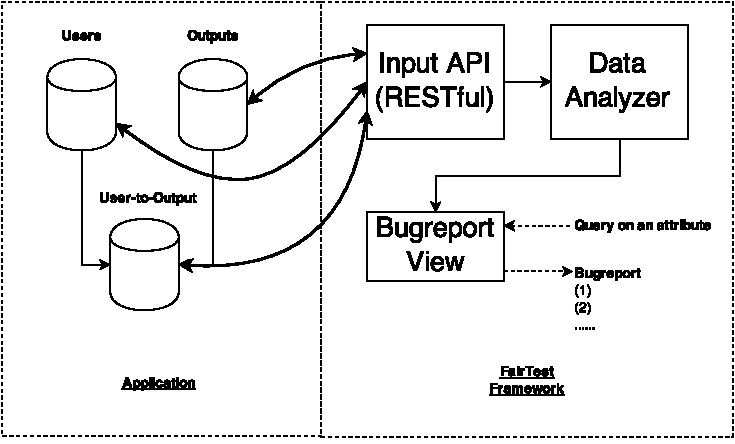
\includegraphics[width=0.49\textwidth]
  {\detokenize{figures/architecture}}
  \caption{{\bf \textit{FairTest}'s Architecture}. The diagram shows \sysname's architecture,
    along with a very simple application using it. Bold lines represent API
    calls and dash lines represent bugreport queries. Solid line indicate data flow
    as part of the application or of the testing framework.}
  \label{fig:FairtestArch}
\end{figure}

%Since \sysname uses a common web framework (Django), it can be
%distributed across a set of servers that share the same database. In this this can
%provide rate-limitation and fault-tolerance in case the system is deployed in
%production and to a large scale. 
%When, at a specific timeframe, the report needs to be shown, the data analyzer
%can be run. 

\subsection{API}
Describe maybe with a table
\begin{itemize}
  \item Describe
  \item Explain why we think it is a good API? (e.g., is it extensible?)
\end{itemize}

The input API consists of several modules for the input info. 
